\section{Perancangan Sistem}
Pada tahap desain, dilakukan:
\begin{itemize}
  \item Perancangan arsitektur sistem yang mengintegrasikan \textit{front-end}, \textit{back-end}, dan layanan AI eksternal.
  \item Perancangan alur proses RAG menggunakan \textit{Langchain}, yang menghubungkan retriever, dokumentasi, dan model LLM.
  \item Desain tampilan antarmuka pengguna (\textit{user interface}) untuk memudahkan mahasiswa dalam mengunggah artikel ilmiah, melakukan interaksi tanya-jawab, membuat sitasi, dan memberi anotasi pada PDF.
  \item Perancangan struktur database menggunakan \emph{PostgreSQL} dan \emph{Redis} untuk menyimpan metadata, histori interaksi, dan catatan pengguna.
\end{itemize}

\subsection{Arsitektur Sistem}
Sistem dirancang dalam arsitektur berbasis layanan terpisah (\textit{modular}) untuk memastikan fleksibilitas dan skalabilitas. Gambar~\ref{fig:arsitektur-sistem} menyajikan arsitektur umum sistem yang dikembangkan.

\begin{figure}[H]
  \centering
  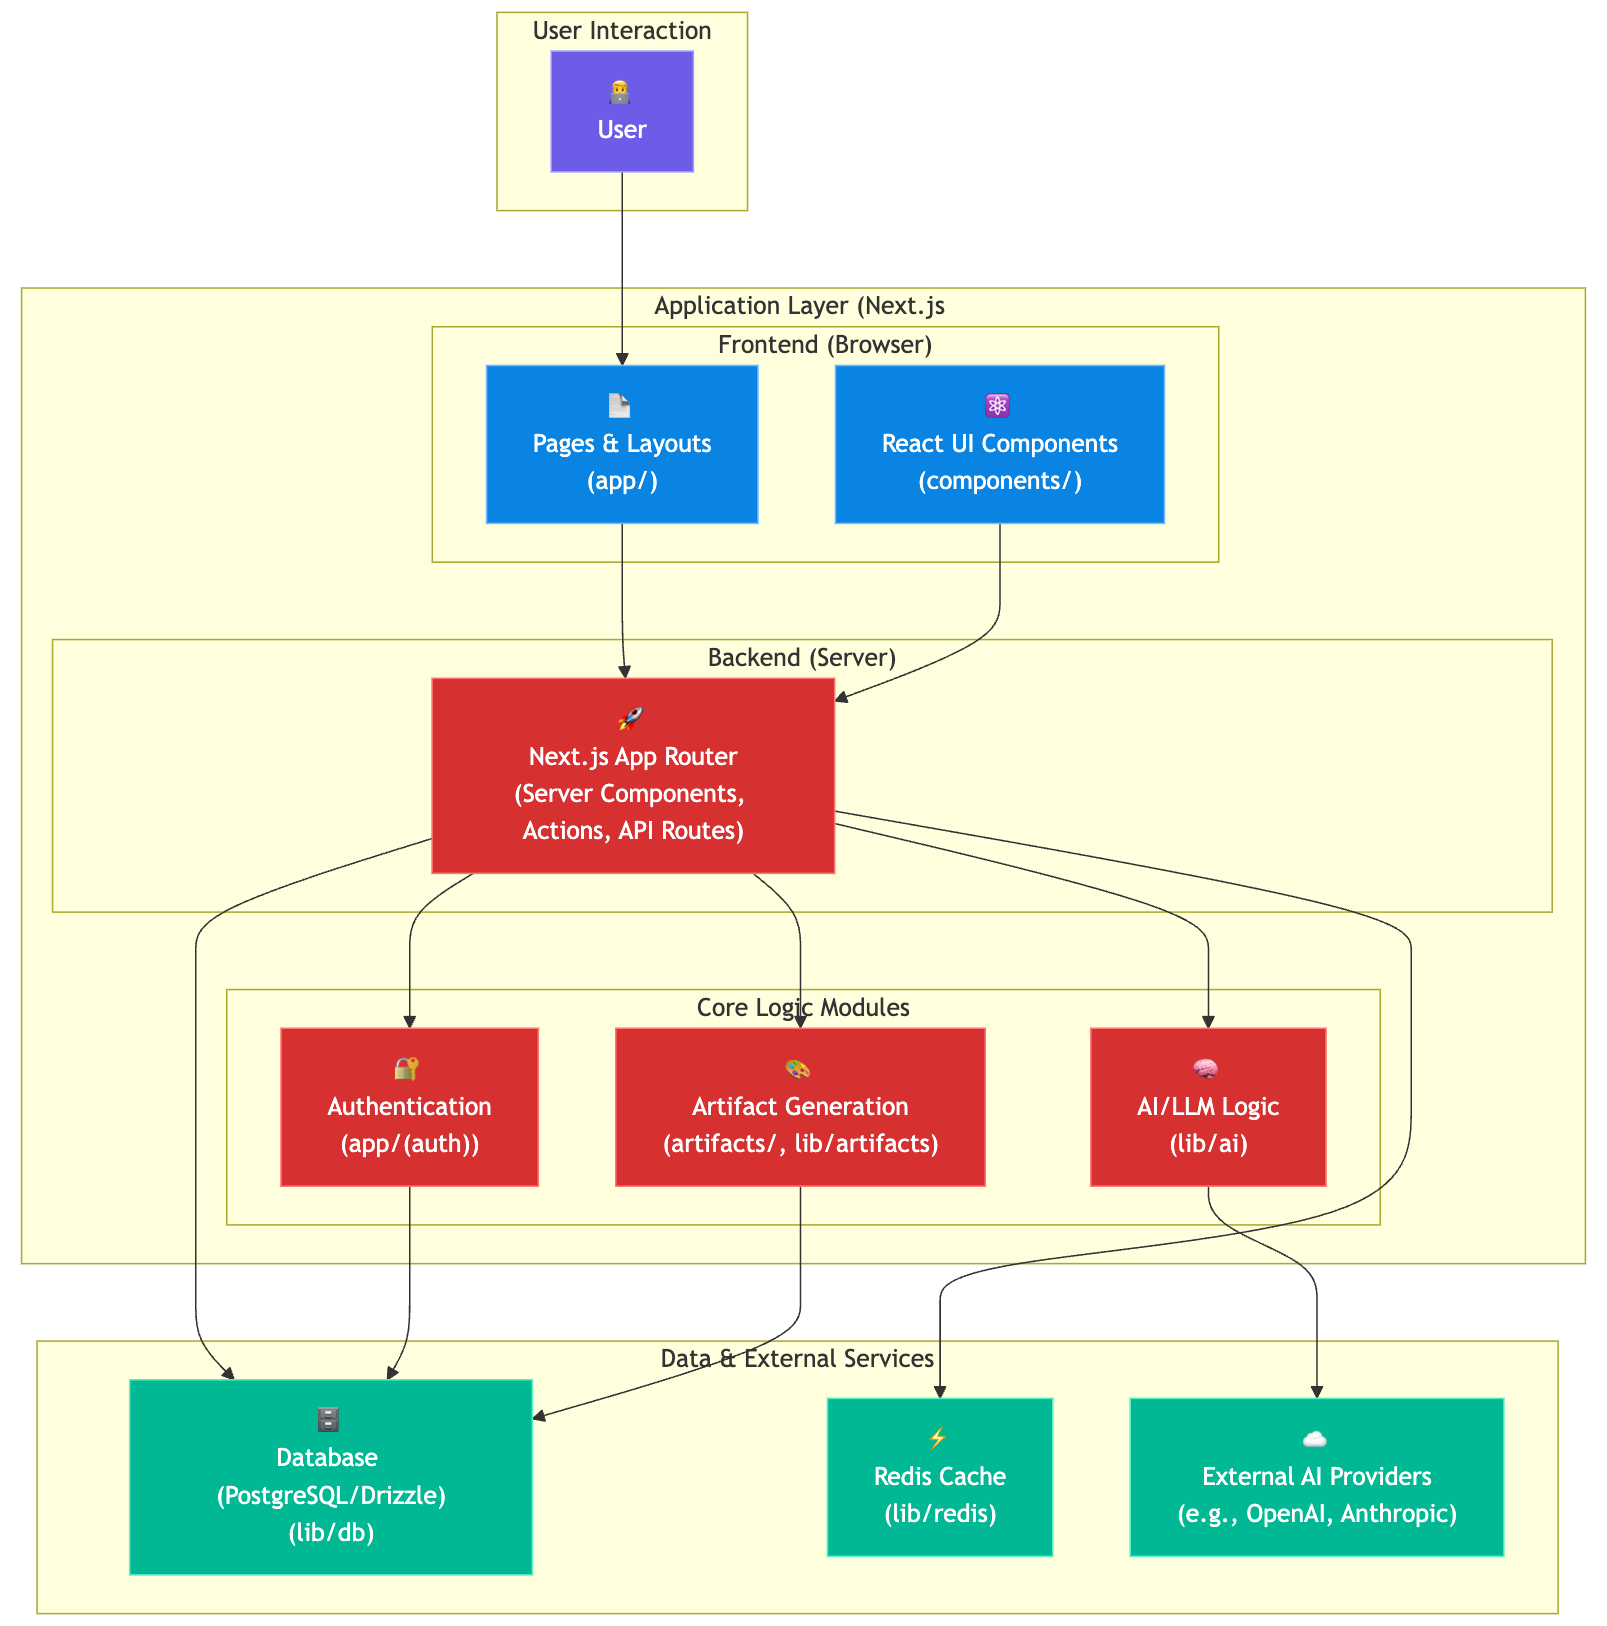
\includegraphics[width=0.9\textwidth]{images/system-arch.png}
  \caption{Arsitektur sistem chatbot dengan RAG dan Langchain}
  \label{fig:arsitektur-sistem}
\end{figure}

\subsection{Use Case Diagram}
Bagian ini menjelaskan fungsionalitas sistem Chatbot Journal dari perspektif pengguna, yang digambarkan melalui use case diagram. Use case diagram ini mengidentifikasi aktor yang berinteraksi dengan sistem dan berbagai fungsi atau layanan yang disediakan oleh sistem.

\begin{figure}[H]
  \centering
  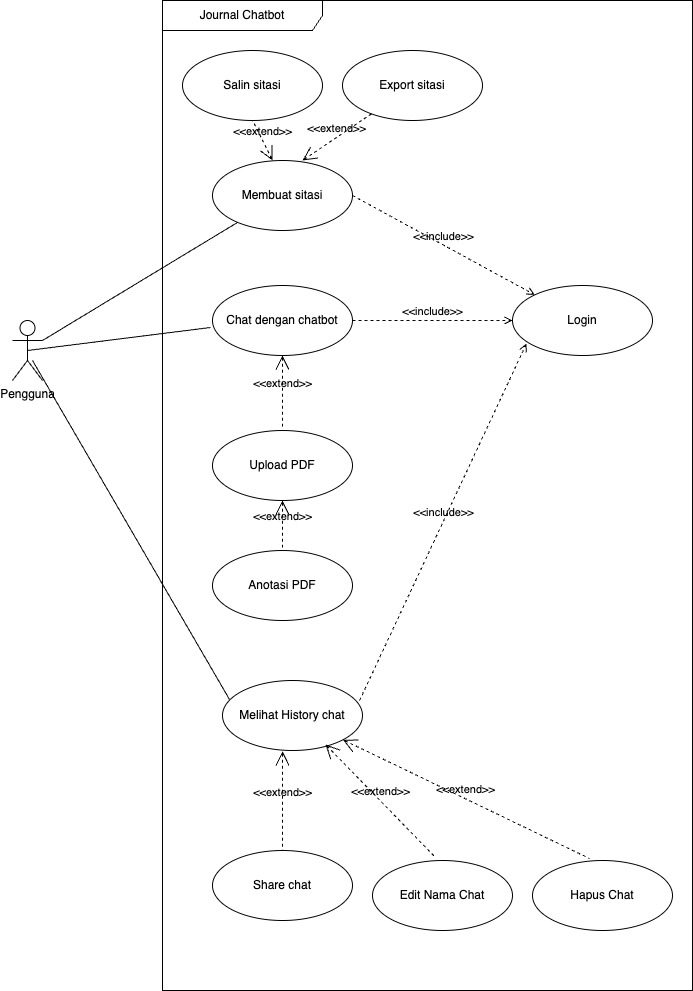
\includegraphics[width=0.9\textwidth]{images/bab-3/usecase.jpg}
  \caption{Use Case Diagram Aplikasi Chatbot Akademik}
  \label{fig:usecase}
\end{figure}
\subsection{Aktor}
Dalam use case diagram ini, terdapat satu aktor utama yaitu \textbf{Pengguna}. Aktor ini merepresentasikan individu yang akan berinteraksi langsung dengan sistem \textit{Journal Chatbot} untuk memenuhi berbagai kebutuhannya terkait manajemen jurnal dan interaksi dengan chatbot.

\subsection{Use Case}
Berikut adalah penjelasan rinci mengenai setiap use case yang terlibat dalam sistem \textit{Journal Chatbot}:

\begin{enumerate}
    \item \textbf{Login}
    \begin{itemize}
        \item \textbf{Deskripsi:} Use case ini memungkinkan pengguna untuk masuk ke dalam sistem dengan menggunakan kredensial yang valid. Ini adalah use case dasar yang harus dilakukan sebelum pengguna dapat mengakses fitur-fitur lain yang memerlukan otentikasi.
        \item \textbf{Relasi:} Use case \textit{Login} di-\textit{include} oleh \textit{Chat dengan Chatbot} dan \textit{Melihat History Chat}, yang berarti setiap kali pengguna ingin melakukan chat atau melihat riwayat chat, mereka harus terlebih dahulu berhasil login.
    \end{itemize}

    \item \textbf{Membuat Sitasi}
    \begin{itemize}
        \item \textbf{Deskripsi:} Use case ini memungkinkan pengguna untuk menghasilkan sitasi dari sumber jurnal atau dokumen yang telah diunggah.
        \item \textbf{Relasi:}
        \begin{itemize}
            \item \textit{Extend Salin Sitasi}: Pengguna dapat memilih untuk menyalin sitasi yang telah dibuat ke clipboard untuk penggunaan lebih lanjut.
            \item \textit{Extend Export Sitasi}: Pengguna dapat memilih untuk mengekspor sitasi ke format lain (misalnya, Bib\TeX, RIS, atau plain text) untuk pengelolaan referensi.
        \end{itemize}
    \end{itemize}

    \item \textbf{Chat dengan Chatbot}
    \begin{itemize}
        \item \textbf{Deskripsi:} Use case ini merupakan inti dari sistem, di mana pengguna dapat berinteraksi secara langsung dengan chatbot untuk mendapatkan informasi, menjawab pertanyaan, atau melakukan tugas-tugas terkait jurnal.
        \item \textbf{Relasi:}
        \begin{itemize}
            \item \textit{Include Login}: Pengguna harus login sebelum dapat berinteraksi dengan chatbot.
            \item \textit{Extend Upload PDF}: Saat berinteraksi dengan chatbot, pengguna memiliki opsi untuk mengunggah dokumen PDF yang kemudian dapat dianalisis atau digunakan oleh chatbot dalam percakapan.
            \item \textit{Extend Anotasi PDF}: Setelah mengunggah PDF, pengguna dapat melakukan anotasi pada dokumen tersebut, seperti menyorot teks, menambahkan catatan, atau menandai bagian-bagian penting. Fitur ini memperkaya interaksi dengan chatbot karena chatbot dapat merujuk pada anotasi pengguna.
        \end{itemize}
    \end{itemize}

    \item \textbf{Melihat History Chat}
    \begin{itemize}
        \item \textbf{Deskripsi:} Use case ini memungkinkan pengguna untuk melihat dan mengelola riwayat percakapan mereka dengan chatbot. Ini sangat penting untuk melacak interaksi sebelumnya dan melanjutkan percakapan.
        \item \textbf{Relasi:}
        \begin{itemize}
            \item \textit{Include Login}: Pengguna harus login untuk dapat mengakses riwayat chat mereka.
            \item \textit{Extend Share Chat}: Pengguna dapat memilih untuk membagikan riwayat chat tertentu dengan pihak lain (misalnya, melalui email atau aplikasi pesan).
            \item \textit{Extend Edit Nama Chat}: Pengguna dapat mengubah nama atau judul dari riwayat chat tertentu untuk mempermudah identifikasi dan pengelolaan.
            \item \textit{Extend Hapus Chat}: Pengguna dapat menghapus riwayat chat yang tidak lagi dibutuhkan untuk menjaga kebersihan data.
        \end{itemize}
    \end{itemize}
\end{enumerate}

\subsection{Relasi Antar Use Case}
\begin{itemize}
    \item \textbf{Relasi \textit{include}}: Menunjukkan bahwa suatu use case menyertakan fungsionalitas dari use case lain secara wajib. Dalam diagram ini, \textit{Login} di-\textit{include} oleh \textit{Chat dengan Chatbot} dan \textit{Melihat History Chat}, yang menekankan bahwa otentikasi adalah prasyarat untuk kedua fungsi tersebut.
    
    \item \textbf{Relasi \textit{extend}}: Menunjukkan bahwa suatu use case dapat memperluas fungsionalitas use case lain dalam kondisi tertentu. Contohnya, \textit{Salin Sitasi} dan \textit{Export Sitasi} adalah opsi tambahan yang tersedia setelah \textit{Membuat Sitasi}. Demikian pula, \textit{Upload PDF} dan \textit{Anotasi PDF} memperluas fungsionalitas \textit{Chat dengan Chatbot}, sementara \textit{Share Chat}, \textit{Edit Nama Chat}, dan \textit{Hapus Chat} memperluas \textit{Melihat History Chat}. Relasi ini menunjukkan fleksibilitas sistem dalam menawarkan fitur tambahan sesuai kebutuhan pengguna.
\end{itemize}

\subsection{Activity Diagram}

Activity Diagram adalah representasi grafis dari alur kerja atau kegiatan di dalam suatu sistem, yang memperlihatkan berbagai langkah yang diperlukan untuk membangun aplikasi chatbot jurnal ini. Berikut merupakan penjelasan lengkap tentang setiap fungsi yang dijalankan sistem ini.

\begin{figure}[H]
  \centering
  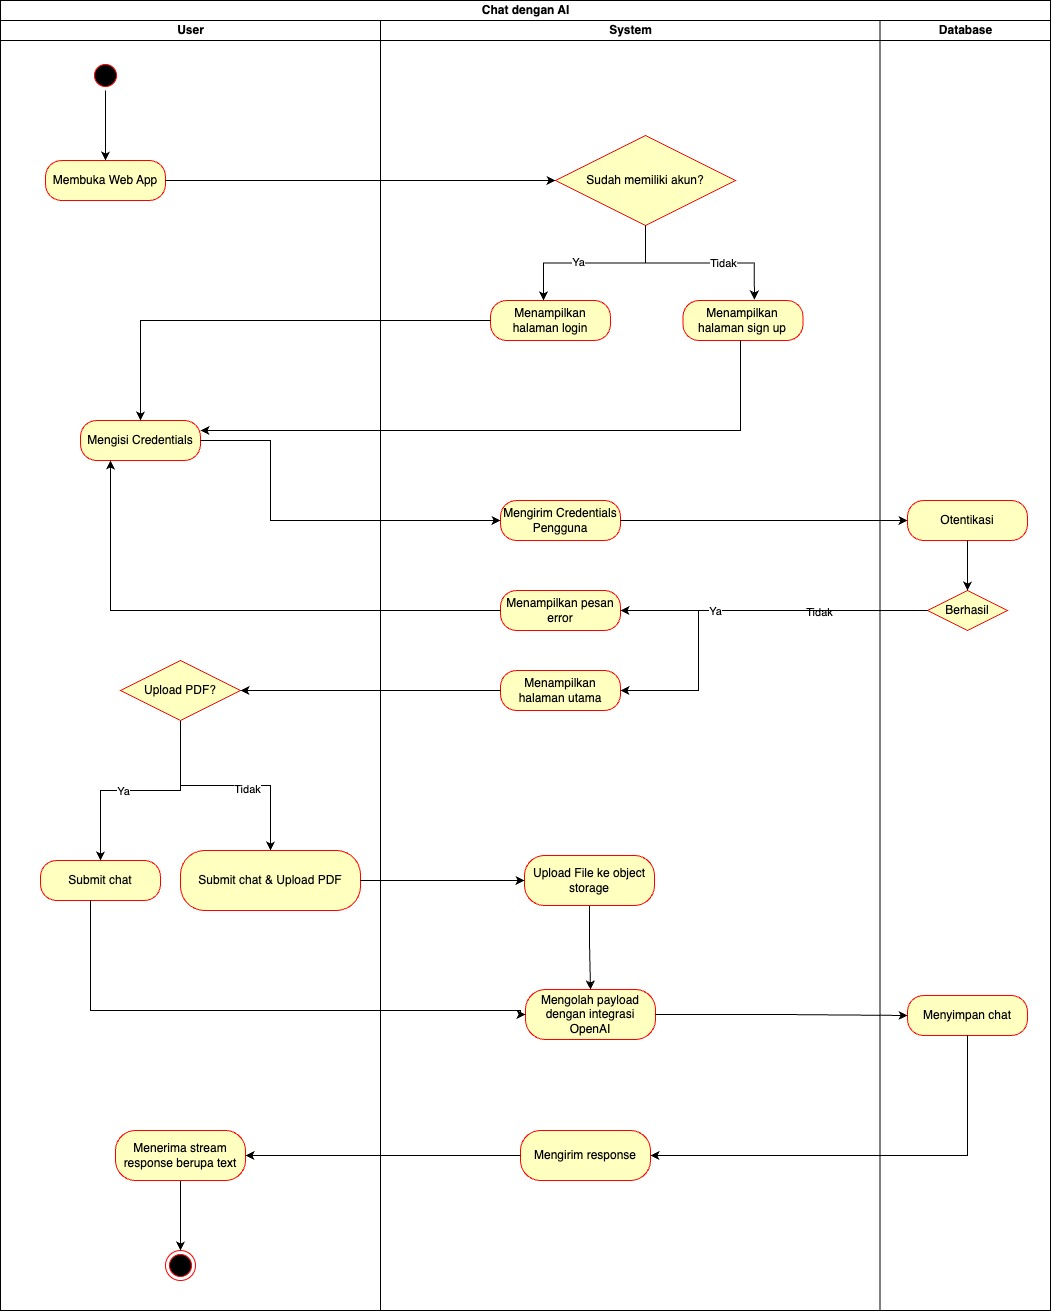
\includegraphics[width=0.9\textwidth]{images/bab-3/sitemap.jpg}
  \caption{Activity Diagram Interaksi Chatbot dengan RAG}
  \label{fig:activity}
\end{figure}

Activity diagram di atas menggambarkan alur proses interaksi pengguna dengan aplikasi. Proses dimulai ketika pengguna membuka web app. Sistem kemudian memeriksa apakah pengguna sudah memiliki akun. Jika belum, sistem akan menampilkan halaman sign up; jika sudah, sistem menampilkan halaman login. Pengguna kemudian mengisi kredensial yang dikirimkan ke sistem untuk proses otentikasi melalui database. Jika otentikasi berhasil, sistem akan menampilkan halaman utama. Jika gagal, sistem akan menampilkan pesan kesalahan.
\singlespacing{}
Setelah berhasil masuk, pengguna dapat memilih apakah ingin mengunggah file PDF atau tidak. Jika tidak, pengguna hanya perlu mengirimkan chat. Namun, jika ingin mengunggah PDF, pengguna akan mengirimkan chat bersamaan dengan file tersebut. File PDF akan diunggah ke object storage, kemudian payload yang berisi chat dan file akan diproses menggunakan integrasi OpenAI.\@ Setelah diproses, hasil response dikirimkan kembali ke sistem dan sistem mengirimkannya ke pengguna dalam bentuk stream teks. Di sisi lain, chat juga disimpan ke dalam database sebagai arsip interaksi.

\subsection{Sequence Diagram}

Gambar~\ref{fig:sequence-login-chat} menunjukkan sequence diagram yang menggambarkan alur interaksi antara pengguna, sistem, dan basis data saat menggunakan aplikasi chatbot jurnal. Diagram ini menjelaskan urutan proses dari mulai membuka aplikasi hingga pengguna menerima respons dari sistem berdasarkan dokumen yang telah diunggah.

\begin{figure}[H]
    \centering
    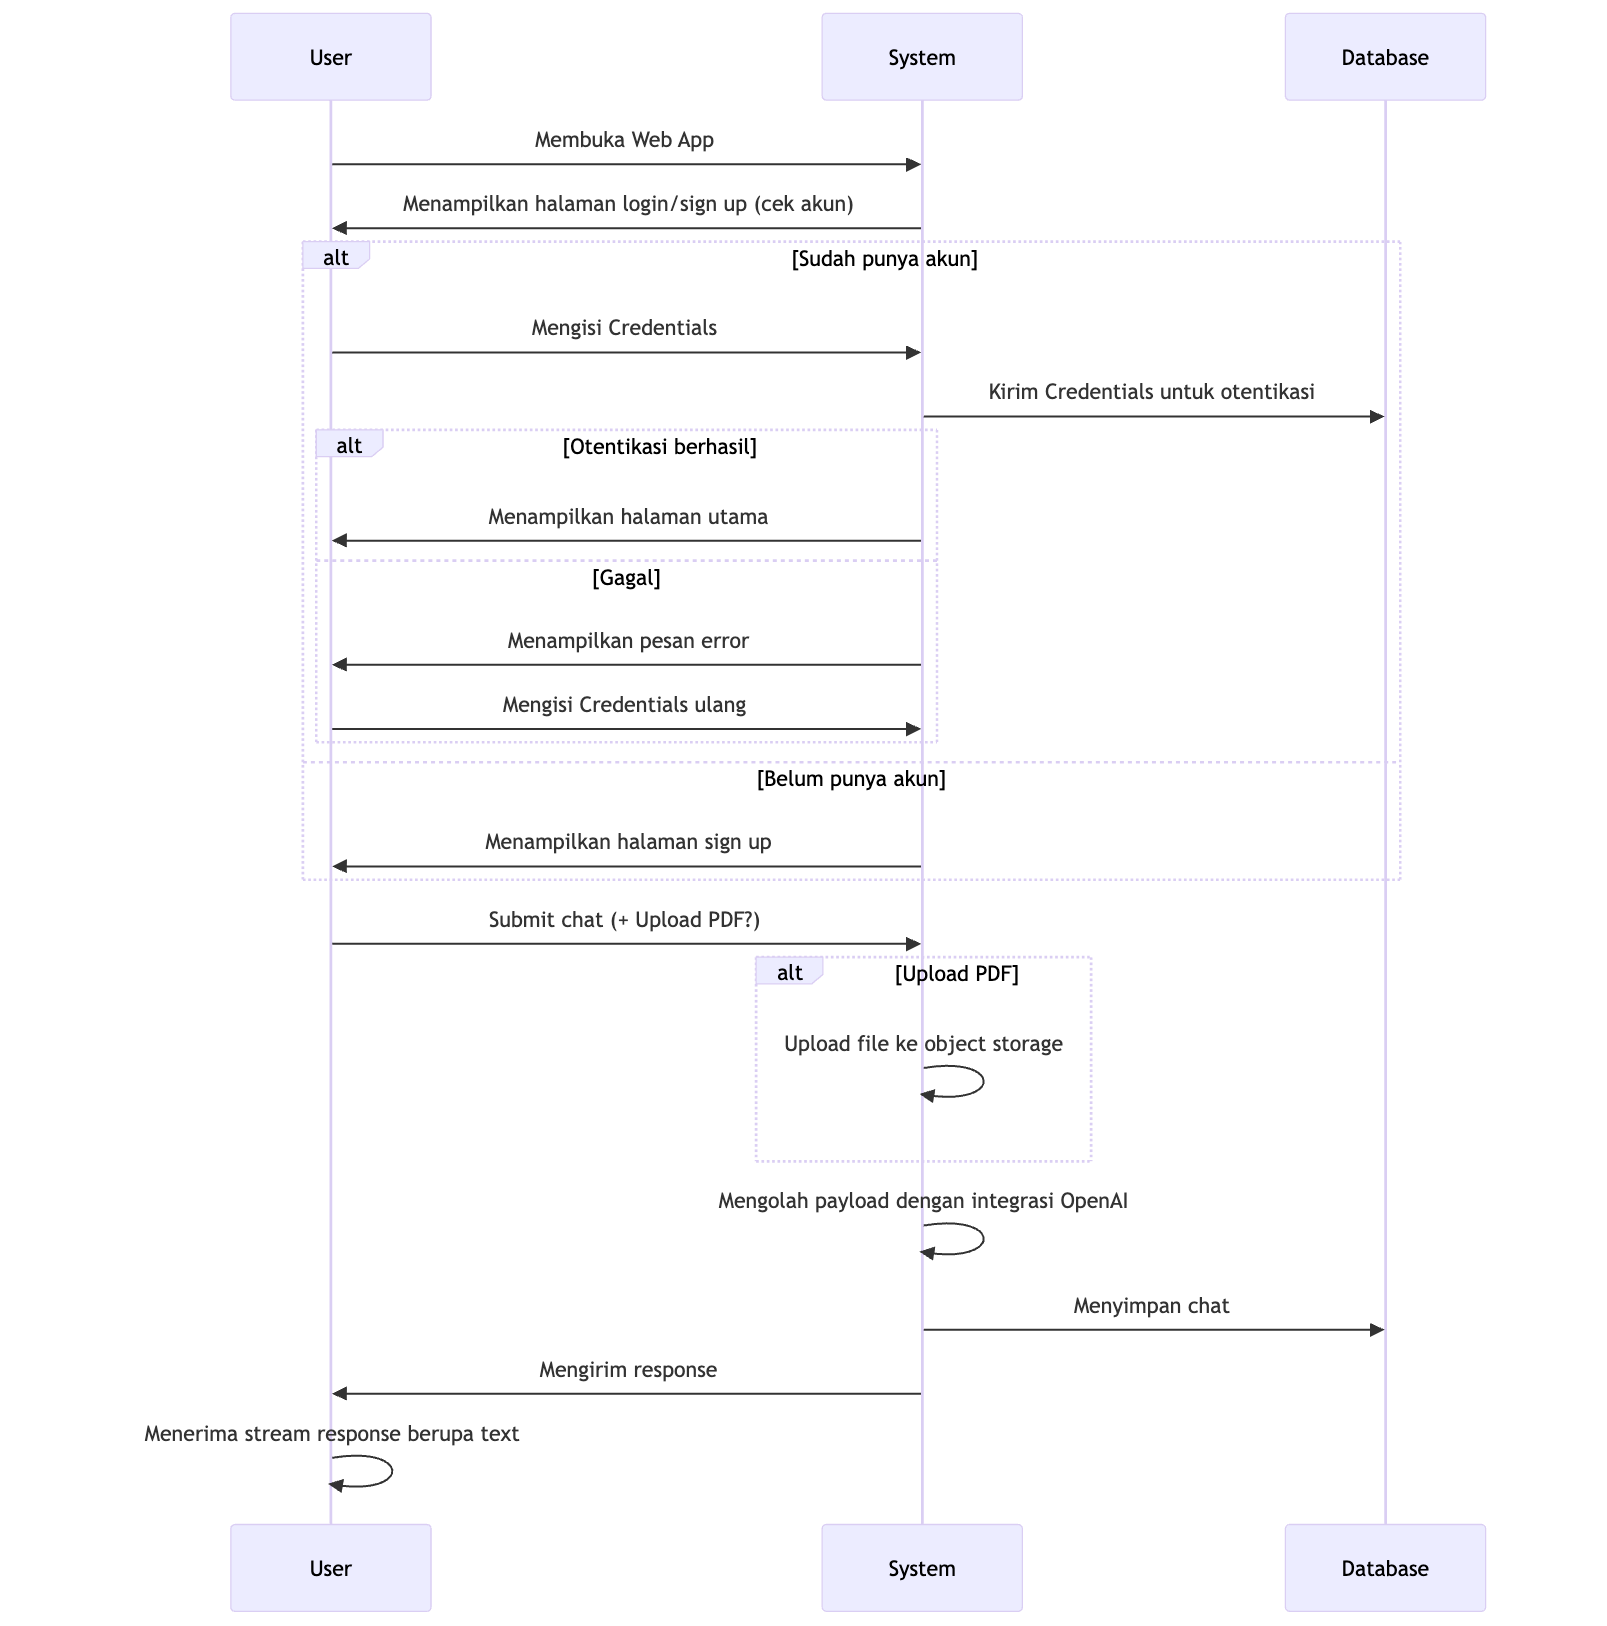
\includegraphics[width=0.9\textwidth]{images/bab-3/sequence.png}
    \caption{Sequence Diagram Interaksi User dan Sistem}
    \label{fig:sequence-login-chat}
\end{figure}

Berdasarkan Gambar~\ref{fig:sequence-login-chat}, berikut adalah tahapan proses yang terjadi:

\begin{enumerate}
  \item \textbf{Pengguna membuka aplikasi web}: Proses dimulai ketika pengguna mengakses aplikasi melalui browser.
  
  \item \textbf{Cek akun dan otentikasi}: Sistem memeriksa apakah pengguna sudah memiliki akun. Jika ya, pengguna mengisi kredensial (email dan password) lalu sistem mengirimkan kredensial tersebut ke backend untuk proses otentikasi.
  
  \item \textbf{Respons otentikasi}: Jika kredensial valid, sistem akan menampilkan halaman utama. Jika tidak, sistem menampilkan pesan error dan meminta pengguna untuk mencoba kembali.
  
  \item \textbf{Registrasi pengguna baru}: Jika pengguna belum memiliki akun, sistem mengarahkan ke halaman sign-up.
  
  \item \textbf{Pengiriman pesan dan dokumen}: Setelah berhasil masuk, pengguna dapat melakukan percakapan dengan chatbot. Jika dibutuhkan, pengguna juga dapat mengunggah file PDF berisi jurnal ilmiah.
  
  \item \textbf{Upload PDF ke Object Storage}: Jika terdapat PDF yang dikirimkan, sistem akan mengunggah file tersebut ke layanan object storage (misalnya Vercel Blob atau storage berbasis cloud lainnya).
  
  \item \textbf{Pemrosesan payload}: Sistem kemudian menggabungkan pertanyaan dan dokumen yang telah diunggah sebagai konteks untuk dikirim ke model LLM (OpenAI GPT-4) melalui integrasi Langchain.
  
  \item \textbf{Penyimpanan riwayat chat}: Setelah mendapatkan hasil respons dari model AI, sistem menyimpan riwayat percakapan (chat) ke basis data untuk kepentingan histori pengguna.
  
  \item \textbf{Streaming respons ke pengguna}: Respons dari model dikirimkan secara bertahap dalam bentuk streaming teks ke pengguna, untuk pengalaman percakapan yang lebih cepat dan real-time.
\end{enumerate}

Diagram ini memvisualisasikan bagaimana sistem menangani proses otentikasi, pengelolaan dokumen, dan integrasi dengan layanan AI secara terstruktur dan efisien. Alur ini juga menunjukkan bahwa sistem bersifat stateless pada sisi server, karena menggunakan pendekatan API tanpa backend server monolitik.

\subsection{Entity Relationship Diagram (ERD)}

Entity Relationship Diagram (ERD) digunakan untuk menggambarkan struktur dan relasi antar tabel dalam basis data aplikasi chatbot berbasis \textit{Retrieval-Augmented Generation (RAG)}. Diagram ini membantu dalam merancang basis data yang efisien dan sesuai dengan kebutuhan fungsional aplikasi.

\begin{figure}[H]
  \centering
  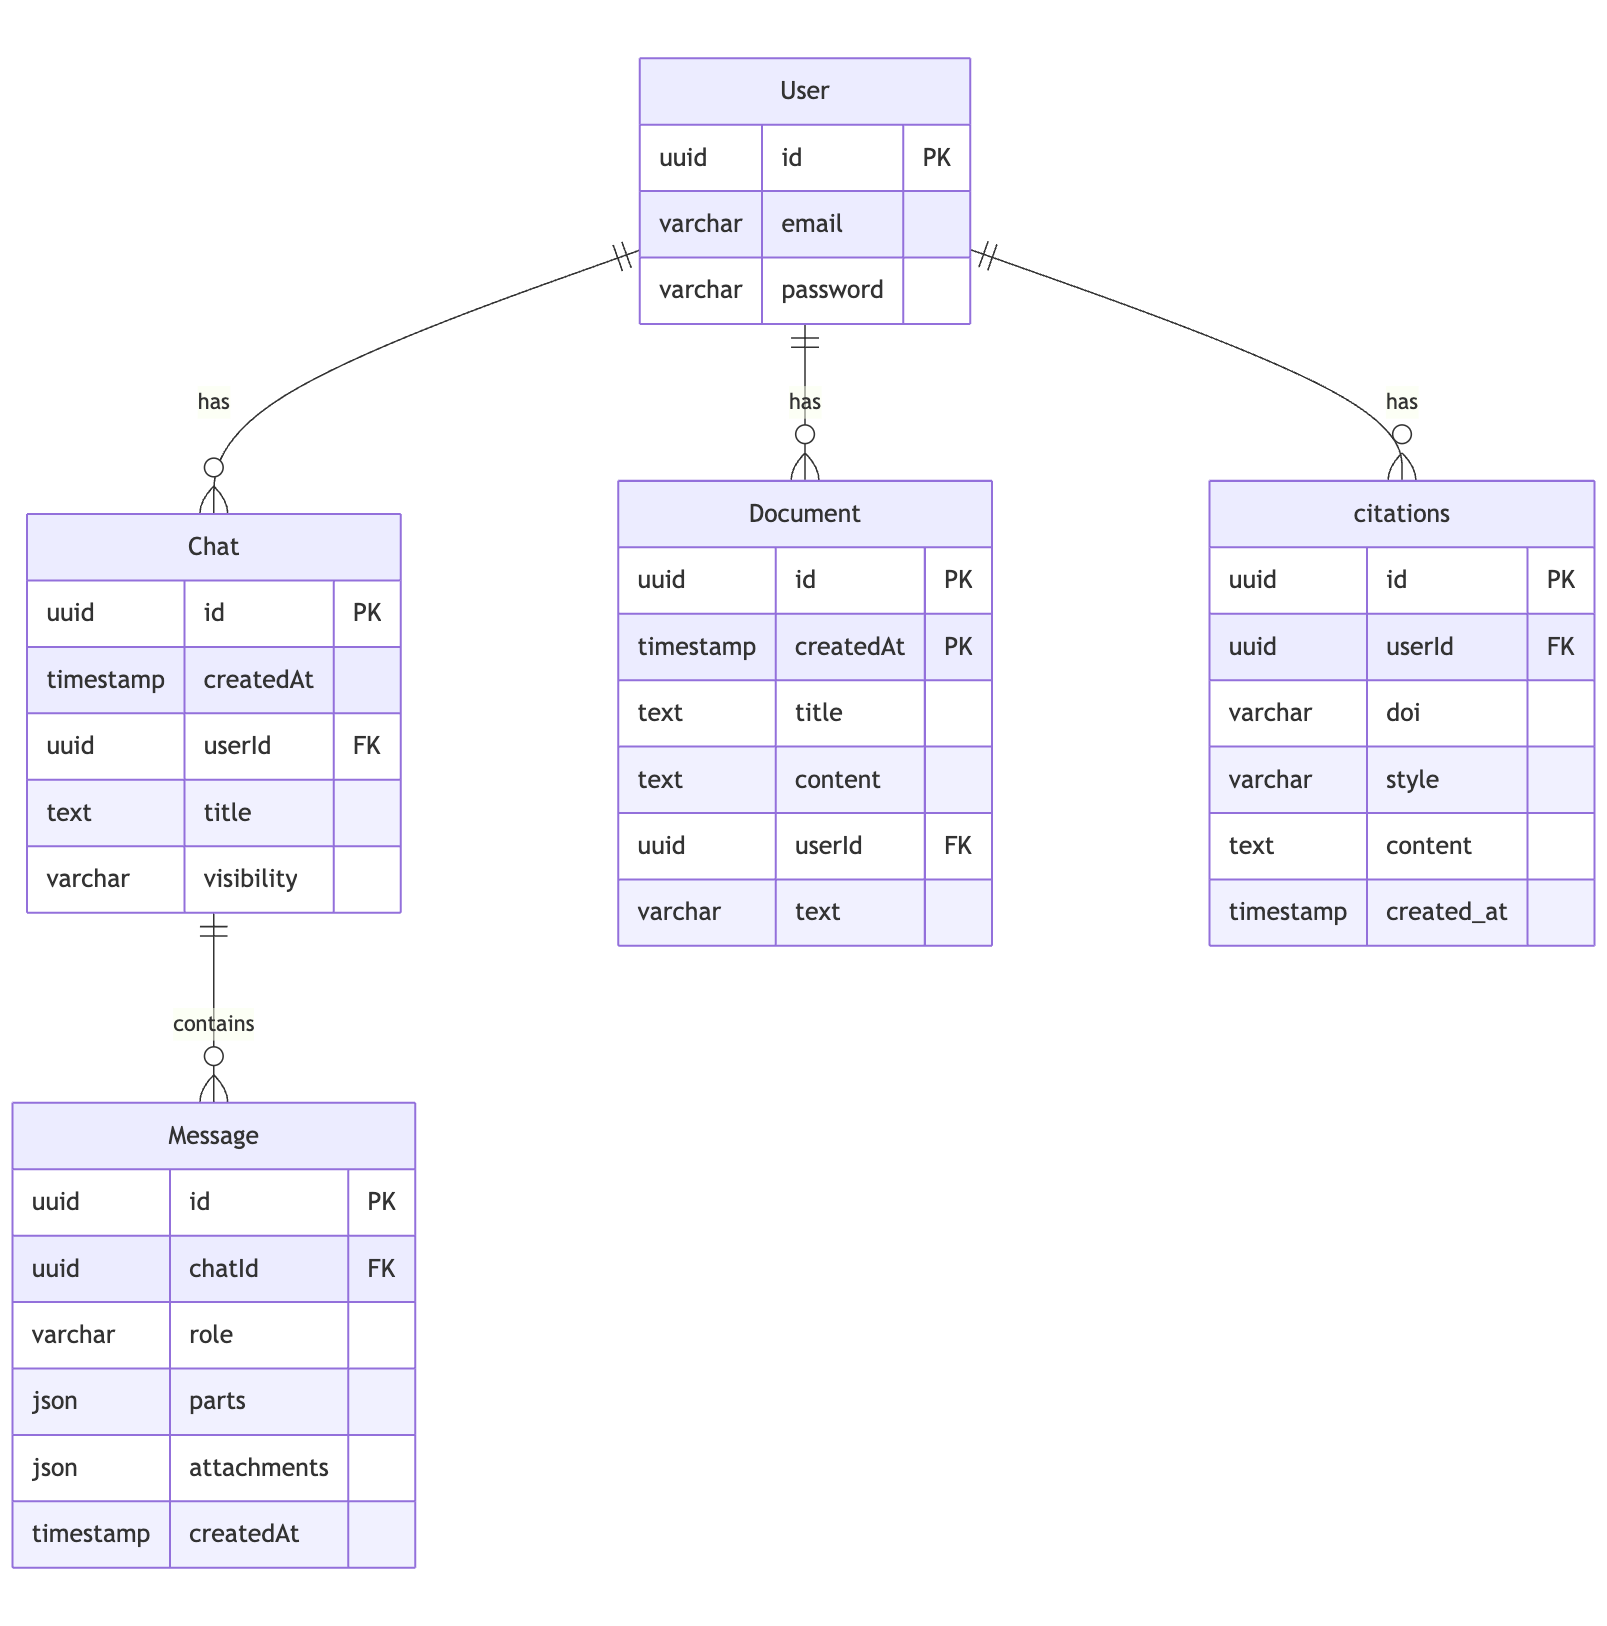
\includegraphics[width=0.95\linewidth]{images/bab-3/erd-skripsi.png}
  \caption{Entity Relationship Diagram Aplikasi}
  \label{fig:erd}
\end{figure}

\noindent Penjelasan masing-masing entitas dalam ERD adalah sebagai berikut:

\begin{itemize}
  \item \textbf{User} \\
  Entitas \texttt{User} menyimpan data pengguna yang terautentikasi. Atribut yang dimiliki:
  \begin{itemize}
    \item \texttt{id}: UUID sebagai \textit{primary key}
    \item \texttt{email}: Alamat email pengguna
    \item \texttt{password}: Kata sandi pengguna (dalam bentuk terenkripsi)
  \end{itemize}
  Relasi: Satu pengguna dapat memiliki banyak \texttt{Chat}, \texttt{Document}, dan \texttt{Citations}.

  \item \textbf{Chat} \\
  Entitas ini merepresentasikan sesi percakapan antara pengguna dan sistem chatbot. Atribut:
  \begin{itemize}
    \item \texttt{id}: UUID sebagai \textit{primary key}
    \item \texttt{createdAt}: Timestamp waktu pembuatan chat
    \item \texttt{userId}: FK mengacu ke \texttt{User}
    \item \texttt{title}: Judul percakapan
    \item \texttt{visibility}: Status visibilitas percakapan (privat/publik)
  \end{itemize}
  Relasi: Satu \texttt{Chat} memiliki banyak \texttt{Message}.

  \item \textbf{Message} \\
  Menyimpan seluruh pesan yang terkandung dalam satu sesi chat. Atribut:
  \begin{itemize}
    \item \texttt{id}: UUID sebagai \textit{primary key}
    \item \texttt{chatId}: FK ke \texttt{Chat}
    \item \texttt{role}: Peran pengirim pesan (user/system)
    \item \texttt{parts}: Konten pesan dalam format JSON
    \item \texttt{attachments}: Lampiran terkait dalam format JSON
    \item \texttt{createdAt}: Timestamp pembuatan pesan
  \end{itemize}

  \item \textbf{Document} \\
  Entitas ini menyimpan data dokumen PDF yang diunggah oleh pengguna. Atribut:
  \begin{itemize}
    \item \texttt{id}: UUID sebagai \textit{primary key}
    \item \texttt{createdAt}: Waktu unggahan dokumen
    \item \texttt{title}: Judul dokumen
    \item \texttt{content}: Isi teks hasil ekstraksi PDF
    \item \texttt{userId}: FK ke \texttt{User}
    \item \texttt{text}: Versi teks tambahan atau metadata (opsional)
  \end{itemize}

  \item \textbf{Citations} \\
  Menyimpan kutipan atau sitasi yang dibuat pengguna berdasarkan dokumen yang telah diunggah. Atribut:
  \begin{itemize}
    \item \texttt{id}: UUID sebagai \textit{primary key}
    \item \texttt{userId}: FK ke \texttt{User}
    \item \texttt{doi}: Digital Object Identifier dari jurnal
    \item \texttt{style}: Gaya kutipan (APA, IEEE, Harvard, dll)
    \item \texttt{content}: Format sitasi lengkap
    \item \texttt{created\_at}: Waktu pembuatan sitasi
  \end{itemize}
\end{itemize}